%********VORAUSSETZUNGEN & GRUNDLAGEN*********
\chapter{Fundumentals}
\label{sec:Fundumentals}
\section{STM-Imaging}
The Scanning Tunneling Microscope was introduced in 1981 by Gerd Binning and Heinrich Roherer. 
With this measuring technique it is possible to resolve a conductive surface with a precission beyond that of conventional light based Microscopes.
In contrast to other electron based microscopy like Scanning Electron Microscopes (SEM) it uses the quantum mechanical phenomenon of tunneling.
In classical mechanics, objects cannot overcome a potential if their energy $E < V_0$, as observed in gravitational interactions.
This phenomenon is observed for quantum mechanical particles like electrons, which can surpass a potential barrier despite the initial expectation that they should not be able to.
The STM uses this effect by precisely positioning a sharp conductive tip close to the surface and applying a bias voltage.
Most STM are operated in Ultra-High-Vacuum (UHV), where the distance between the tip and the surface represents the tunneling barrier.
By varying the bias voltage, the tunneling probability can be changed, thereby affecting the tunneling current.
If the bias voltage, also referred to as the potential difference, is kept constant, the tunneling current is primarily dependent on the distance between tip and surface.
The tip is moved in the x-,y-plane where a grid is established. 
There are two modes of operation, the constant-height and the constant-current mode.
The latter is especially useful for irregular surfaces, because the tip is moved up and down to keep the tunneling current constant.
The movement signal of the piezos is then converted into height.
In constant-height mode the position of the tip stayes fixed and the tunneling current $I_t$ is measured and converted into height information. \\

\newpage
\begin{wrapfigure}{r}{0.5\textwidth}
    \centering
    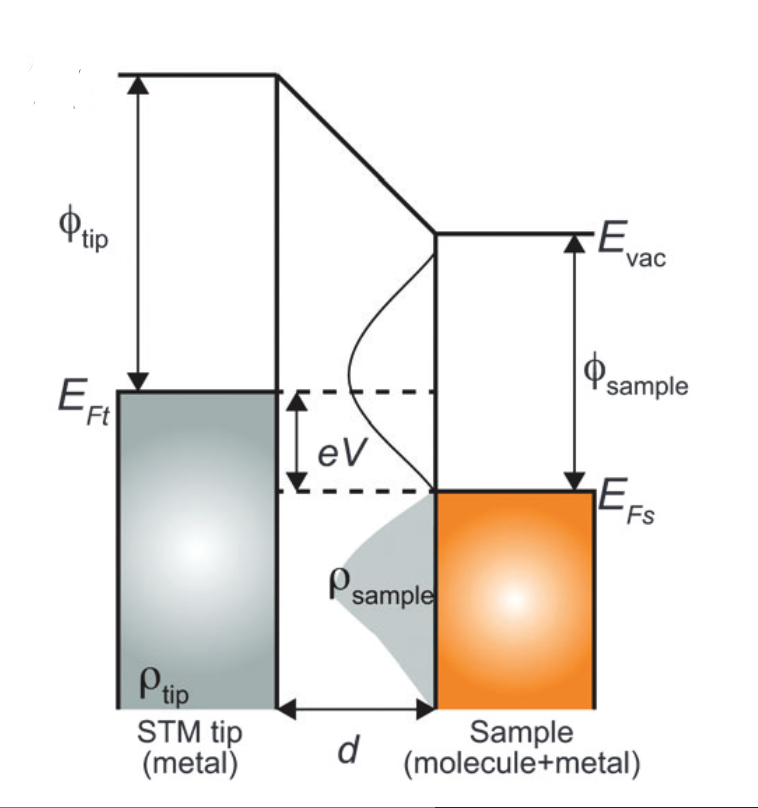
\includegraphics[width=0.4\textwidth]{graphics/Tunneling_diagram_japan.PNG}
    \caption{Energy diagram of the tunneling junction with a positive bias voltage applied. $\Phi_{tip}$ \& $\Phi_{sample}$: working functions of either tip and sample, $E_{vac}$: vacuum energy level,  $E_{ft}$ \& $E_{fs}$: Fermi Energys of the tip and sample,  $\rho_{tip}$ \& $\rho_{sample}$: density of states of tip and sample,  $eV$: potential difference caused by applying a bias Voltage $V$ (picture source: \cite{Kano}) }
    \label{fig:energy_diagram}
\end{wrapfigure}

The tunneling current, at a arbituery gridpoint, is influenced by the electronic structure of the tip and sample.
If the tip is in vicinity of the metallic substrate the fermi energies align, resulting in an equal probability of electrons tunneling from the tip to the sample and vice versa.
This consequently results in a zero net current. 
Through the introduction of a electric potential $V_{bias}$ the fermi energies of tip and sample can be shifted relative to each other (Figure \ref{fig:energy_diagram}).
If the bias voltage is positive the fermi energy of the sample is pushed down and electrons from occupied states in the tip can tunnel into the empty states of the sample.
Consequently if the bias voltage is negative electrons from the filled states of the sample tunnel into the tip.
The tunneling current is influenced by the distance $d$ between orbitals of the tip and the sample, which makes it possible to gain information about the electronic structure of the sample.
This is not really a representation of the real structure of the atoms or molecules, but the Local Density of States (LDOS) of the sample´s surface.
Utilizing this in Scanning Tunneling Spectroscopy (STS) provides additional information beyond the sample's topography.
Such as the chemical composition, bonding, the energy gap and band-bending effects \cite{cbai}.
\section{Mathematical Foundation}
\begin{wrapfigure}{r}{0.3\textwidth}
    \centering
    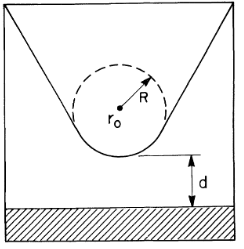
\includegraphics[width=0.3\textwidth]{graphics/fundamental_tip_sheme.PNG}
    \caption{Schematic depiction of the tip geometry \cite{PhysRevLett}}
    \label{fig:tip_scheme}
\end{wrapfigure}
To understand the tip sample interaction one must look at the quantum-mechnical Foundation behind it.
At its simplest the tip can be approximatated as spherical potential well (Figure \ref{fig:tip_scheme}). $R$ is in that case the radius of the tip located at position $\vec{r_0}$ with the distance $d$ from the surface.
First order pertubation theory gives the following expression (Eq. \ref{eq:tunneling_pert}) for the tunneling current of this system \cite{PhysRevLett}:
\begin{equation}
    I = \frac{2 \pi e}{\hbar} \sum_{\mu \nu} f(E_{\mu})[1 - f(E_{\nu}+eV_{bias})]\cdot |M_{\mu \nu}|^2 \delta(E_{\mu}- E_{\nu})
    \label{eq:tunneling_pert}
\end{equation}
\newpage

The fermi distribution $f(E)= (\exp((E-E_F)/k_b T)+1)^{-1}$ gives the ocupation probability of a fermion (electrons) with the Energy $E$ near the fermi level.
In this case it is the ocupation probability of the tip states (denoted by the subindex $\mu$) and the ocupation probability of the sample states ( denoted by the subindex $\nu$).
The tunneling matrix $M_{\mu \nu}$ is related to the derivatives of the sample wave functions $\psi_{\nu} $ at the nucleus of the apex atom \cite{tunnelmatrix}.
Because the STM Imaging is done at low temperatures and with small voltages the Equation \ref{eq:tunneling_pert} can be simplified to:
\begin{equation}
    I = \frac{2 \pi}{\hbar} e^2 V_{bias} \sum_{\mu \nu}  |M_{\mu \nu}|^2 \delta(E{\nu}-E_F) \delta(E_{\mu}- E_{F})
    \label{eq:tunneling_pert_simple}
\end{equation}